\section{Durchführung}
\label{sec:Durchführung}
Zur Messung der Absorption der $\beta$- und $\gamma$-Strahlung wird ein Geiger-Müller-Zählrohr innerhalb einer Beliabschirmung gegenüber einer Strahlungsquelle, vor
welcher das entsprechende Absorbermaterial platziert wurde, genutzt. Dies ist schmeatisch in Abbildung \ref{fig:Aufbau} dargestellt.
\begin{figure}
  \centering
  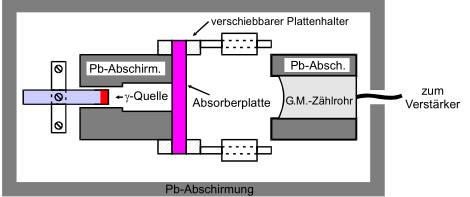
\includegraphics{pictures/Aufbau.png}
  \caption{Schematischer Aufbau der Messapparatur für Gammstrahlung.\cite{sample}}
  \label{fig:Aufbau}
\end{figure}
Das Zählrohr wird dabei über einen Verstärker an ein elektronisches Zählwerk angeschlossen, welches die Messzeit über die Netzfrequenz festlegt.
Nun wird zunächst ohne Strahlungsquelle und Absorber eine Nullmessung der Hintergrundstrahlung über $\SI{900}{\second}$ durchgeführt.
Danach wird für den $\gamma$-Strahler einmal für Blei und einmal für Zink die Counts und die Absorberdicke gemessen.
Dabei wird folgendermaßen vorgegangen. Es werden zunächst mehrere Platten des Absorbermaterials, deren Dicken vorher mittels Schieblehre gemessen wurden,
hintereinander eingespannt, bis die maximal zu messende Schichtdicke erreicht ist. Dann werden die Counts über einen ausreichend langen Zeitraum gemessen, eine Platte
entfernt und erneut gemessen. Dies wird wiederholt bis kein Absorber mehr vorhanden ist und anschließend wird noch eine Messung ohne Absober gemacht.
Die Messung für die $\beta$-Strahlung verläuft analog, nur dass hierbei nicht mit mehreren Platten hintereinader, sondern mit verschieden dicken Platten, welche
nacheinander gemessen werden gearbeitet wird. Das zu messende Absorbermaterial ist in diesem Fall Aluminium.
